\documentclass[12pt]{article}
\usepackage[utf8]{inputenc}
\usepackage{amsmath}
\usepackage{amssymb}
\usepackage{graphicx}
\usepackage{pgfplots}
\usepackage[margin=1in]{geometry}
\newcommand{\x}{\cdot}
\newcommand{\eval}[3]{\left.#1\right\rvert_{#2}^{#3}}
\newcommand{\nroot}[2]{\sqrt[\leftroot{-1}\uproot{1}#1]{#2}}
\newcommand{\paren}[1]{\left(#1\right)}
\newcommand{\braks}[1]{\left[#1\right]}
\newcommand{\curly}[1]{\left\{#1\right\}}
\newcommand{\norm}[1]{\lVert#1\rVert}
\newcommand{\inner}[2]{\langle#1,#2\rangle}
\newcommand{\argmax}[1]{\underset{#1}{\operatorname{arg\,max\,}}}
\newcommand{\argmin}[1]{\underset{#1}{\operatorname{arg\,min\,}}}

\tikzset{
	jumpdot/.style={mark=*,solid},
	excl/.append style={jumpdot,fill=white},
	incl/.append style={jumpdot,fill=blue},
}

\begin{document}

\begin{center}
	\LARGE{Logistic Regression}
\end{center}

\section{Hypothesis}

Consider the domain $\mathcal{X} = \mathbb{R}^D$ and the codomain  $\mathcal{Y} = \{0, 1\}$. In Logistic Regression, we are trying to find an optimal hypothesis $h_{\theta} : \mathcal{X} \rightarrow [0, 1]$ in the hypothesis class
\[ \mathcal{H} = \curly{ h_{\theta} : h_{\theta}(\mathbf{x}) = \sigma(\theta^\top\mathbf{x}) = \frac{1}{1 + e^{-\theta^\top\mathbf{x}}}} \]
which maximizes the likelihood that data is classified correctly. Note that the output of the hypothesis is a real number (i.e. $h_{\theta}(\mathbf{x}) \in [0, 1]$). Thus, a threshold must be applied to $h_\theta(\mathbf{x})$ to obtain actual labels. This is related to why Logistic \textit{Regression} is actually used for classification: even though our final output is a binary label through the use of a threshold, we are still performing regression to find the optimal hypothesis first.
\\\newline
The function $\sigma$ above is called the logistic or sigmoid function, and is used because we want to model the probability that some data point $\mathbf{x}$ has label $y$. This probability can be expressed through the Bernoulli distribution, since labels are binary, like so
\[ p(y \mid \mathbf{x}; \theta) = h_\theta(\mathbf{x})^y(1 - h_\theta(\mathbf{x}))^{1-y} \]
Thus, we can use the logistic function to know the probability that the label is $1$. Namely, we have that $p(y = 1 \mid \mathbf{x}; \theta) = h_\theta(\mathbf{x}) = \sigma(\theta^\top\mathbf{x})$, and therefore also that $p(y = 0 \mid \mathbf{x}; \theta) = 1 - h_\theta(\mathbf{x}) = 1 - \sigma(\theta^\top\mathbf{x})$. This allows us to derive a likelihood function for the hypothesis with regards to the data, given by
\[ \mathcal{L}(h_\theta; S) = \prod_{i=1}^{N}p(y_i \mid \mathbf{x}_i; \theta) \]
By negating the function and taking its log, we obtain an objective function which we can minimize (which is equivalent to maximizing the original likelihood function) in order to find the optimal hypothesis (which would maximize the likelihood given by the original functional). We denote this new objective function by $NLL(h_\theta;S) = -\log\mathcal{L}(h_\theta; S)$.

\section{Gradient Descent}

Gradient descent is an efficient optimization option for finding the optimal hypothesis since $NLL(h_\theta; S)$ only has one global minima its gradient is quite simple. It is given by
\[ \nabla_\theta NLL(h_\theta; S) = \sum_{i=1}^{N}(h_\theta(\mathbf{x}_i) - y_i)\mathbf{x}_i \]
By defining the matrices $X$, $Y$ and $\mathbf{h}_\theta$ as such
\[
	X =
	\begin{bmatrix}
		- \; \mathbf{x}_1 \; - \\
		- \; \mathbf{x}_2 \; - \\
		\vdots \\
		- \; \mathbf{x}_N \; -
	\end{bmatrix}
	, \quad
	Y =
	\begin{bmatrix}
		\; y_1 \; \\
		\; y_2 \; \\
		\vdots \\
		\; y_N \;
	\end{bmatrix}
	, \quad
	\mathbf{h}_\theta =
	\begin{bmatrix}
		h_\theta(\mathbf{x}_1) \\
		h_\theta(\mathbf{x}_2) \\
		\vdots \\
	\end{bmatrix}
\]
we can rewrite the gradient using matrix operations, as such
\[ \nabla_\theta NLL(h_\theta; S) = X^\top(\mathbf{h}_\theta - Y) \]

\section{Regularization}

If data is linearly separable, gradient descent will ``push" $\norm{\theta}$ to infinity in order to make $p(y_i \mid \mathbf{x}_i; \theta)$ approach $1$. The larger $\norm{\theta}$ is, the ``sharper" the logistic curve is, as illustrated by the one-dimensional example below
\begin{center}
	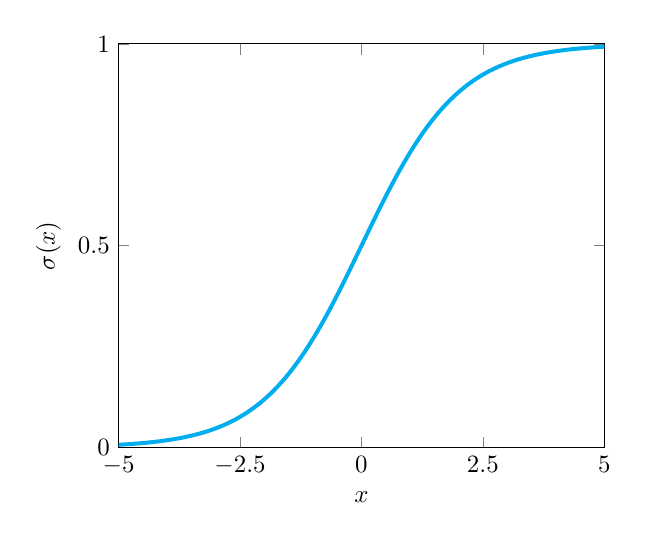
\begin{tikzpicture}[scale=0.9]
		\begin{axis} [
		xtick={-5,-2.5,0,2.5,5},
		ytick={0,0.5,1},
		xlabel={$x$},
		ylabel={$\sigma(x)$},
		xmin = -5, xmax = 5,
		ymin = 0, ymax = 1,
		samples = 100]
		\addplot [cyan, ultra thick, domain = -5.1:5.1] {1/(1+e^-x)};
		\end{axis} 
	\end{tikzpicture}
	\quad
	\begin{tikzpicture}[scale=0.9]
		\begin{axis} [
		xtick={-5,-2.5,0,2.5,5},
		ytick={0,0.5,1},
		xlabel={$x$},
		ylabel={$\sigma(10x)$},
		xmin = -5, xmax = 5,
		ymin = 0, ymax = 1,
		samples = 100]
		\addplot [cyan, ultra thick, domain = -5.1:5.1] {1/(1+e^-10*x)};
		\end{axis} 
	\end{tikzpicture}
\end{center}
With $\norm{\theta}$ at infinity, a sharp ``division" is created, and all $p(y_i \mid \mathbf{x}_i; \theta) = 1$.
\\\newline
Thus, it is important to regularize the objective function to avoid this issue. To accomplish this, ridge regression can be used. The new objective function then becomes
\[ NLL(h_\theta; S) + \lambda\norm{\theta}^2 \]
and its gradient, which can be used in gradient descent, is
\[ X^\top(\mathbf{h}_\theta - Y) + \lambda\theta \]

\end{document}

